\documentclass[conference]{IEEEtran}
% \IEEEoverridecommandlockouts
% The preceding line is only needed to identify funding in the first footnote. If that is unneeded, please comment it out.
\usepackage{cite}
\usepackage{amsmath,amssymb,amsfonts}
\usepackage{algorithmic}
\usepackage{graphicx}
\usepackage{listings}
\usepackage{textcomp}
\usepackage{xcolor}
\def\BibTeX{{\rm B\kern-.05em{\sc i\kern-.025em b}\kern-.08em
		T\kern-.1667em\lower.7ex\hbox{E}\kern-.125emX}}
\begin{document}
	
	\title{2Jason4JSON: A Multi-Agent Team for RoboCup}
	
	\author{\IEEEauthorblockN{Taylor Abraham}
		\IEEEauthorblockA{\textit{Systems and Computer Engineering} \\
			\textit{Carleton University}\\
			Ottawa, Canada \\
			taylorabraham@cmail.carleton.ca}
		\and
		\IEEEauthorblockN{David Bascelli}
		\IEEEauthorblockA{\textit{Systems and Computer Engineering} \\
			\textit{Carleton University}\\
			Ottawa, Canada \\
			davidbascelli@cmail.carleton.ca}
		\and
		\IEEEauthorblockN{Joshua Fryer}
		\IEEEauthorblockA{\textit{Systems and Computer Engineering} \\
			\textit{Carleton University}\\
			Ottawa, Canada \\
			joshfryer@cmail.carleton.ca}
		\and
		\IEEEauthorblockN{Zein Hajj-Ali}
		\IEEEauthorblockA{\textit{Systems and Computer Engineering} \\
			\textit{Carleton University}\\
			Ottawa, Canada \\
			zeinhajjali@cmail.carleton.ca}
	}
	
	\maketitle
	
	\begin{abstract}
		A team of Robocup soccer-playing agents was implemented using the Jason framework\footnote{http://jason.sourceforge.net/wp/}, creating a team of five Jason agents which communicate with each other and execute plans; these agents perceived and acted upon the virtual soccer field by interfacing with Krislet entities. The team demonstrated cooperative behaviour in scoring on the opposing net and preventing scoring on the friendly net.
	\end{abstract}
	
	\section{Introduction}
	Our goal was to design and implement a multi-agent system of agents that communicate and exhibited coordination to (reasonably) successfully play soccer in the Robocup soccer simulation. Jason was chosen as the framework because it extends the already-useful AgentSpeak language’s basis for belief-desire-intention (BDI) programming with inter-agent communication and a shared abstract environment to help manage the agents’ percepts and execute their actions. 
	
	\section{Design}
	
	\subsection{BDI Architecture}
	Our agents use a Belief-Desire-Intention (BDI) design; they hold beliefs (things they know about the world and themselves, such as their position relative to objects, or messages they have been given by other agents), desires or goals (a collection of beliefs they wish to hold and maintain, such as having kicked the ball towards the opposing net), and intentions or plans to reach those goals given their current set of beliefs. 
	\begin{figure}[ht]
		\centering
		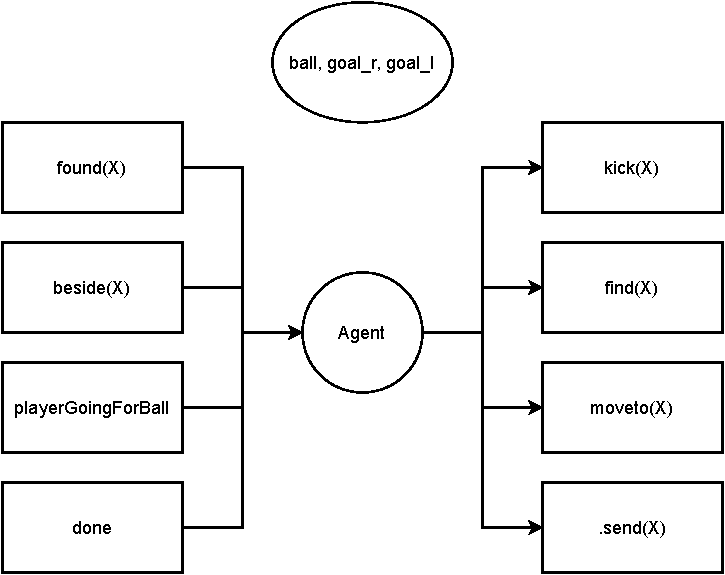
\includegraphics[scale=0.5]{fig/percepts-and-actions.pdf}
		\caption{Some key percepts and actions used in our agents}
		\label{percepts-actions}
	\end{figure}
	
	
	\subsection{Goals and Planning}
	
	We designed two types of player agent, to fulfill different roles: offensive players ("strikers"), and defensive players ("defenders"). Their decision processes are as follows:
	
	\subsubsection{Strikers}
	The first striker to see the ball takes on the role of primary attacker, and attempts to kick the ball into the net. It notifies the other strikers of this, and they take on an assisting role and run towards the opposing net. When the attacking striker kicks, it notifies all strikers that it has done so, and the role assignment happens again. Figure \ref{sequence-diagram} is a sequence diagram illustrating the interplay and communication of the striker agents.
	\begin{figure}[ht]
		\centering
		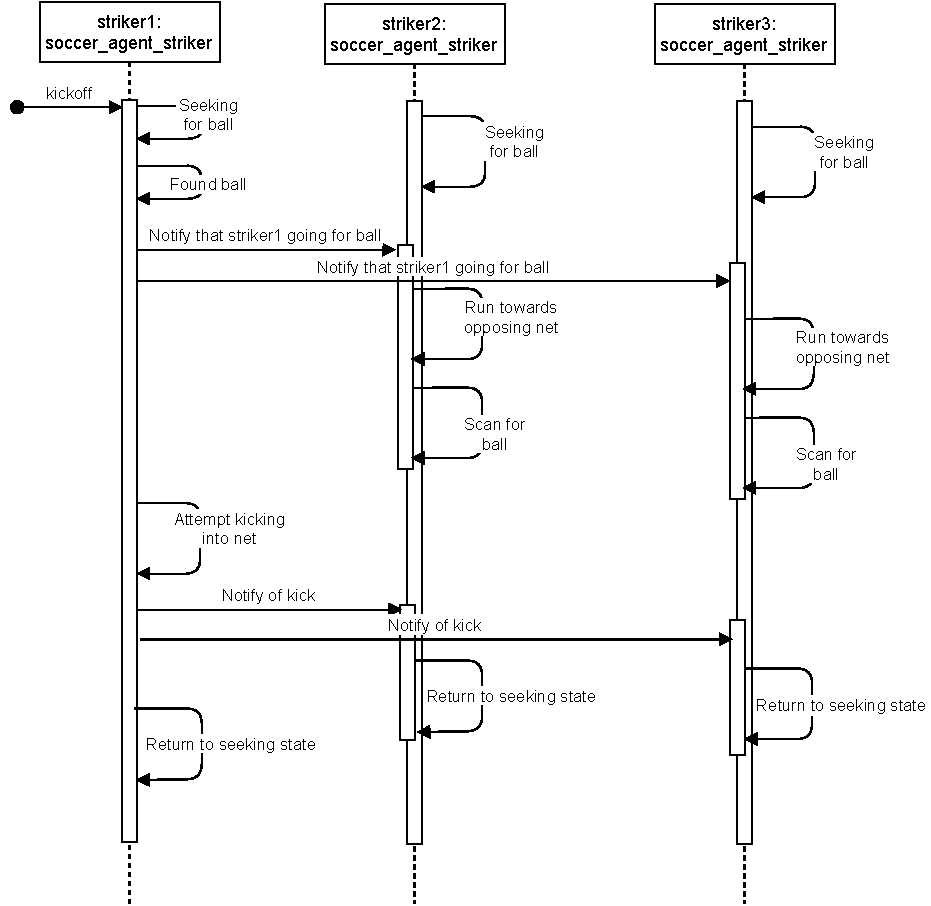
\includegraphics[scale=0.5]{fig/sequence-diagram.pdf}
		\caption{Communication between striker-type agents}
		\label{sequence-diagram}
	\end{figure}
	
	\subsubsection{Defender}
	Each defender looks for their own net and runs towards it. Once they are near the net, they then defend the net by searching for the ball and, if the ball is within a certain distance of them, approaches the ball and kicks it away towards the opposing net.
	
	
	\section{Implementation}
	Three discrete components are involved in controlling agents: the Jason framework, the Java environment, and the Krislet player. 
	
	\subsection{Jason}
	The abstract player behaviours were first formalized in flowcharts (Figure \ref{flowchart-striker}, Figure  \ref{flowchart-defender}), and then adapted into AgentSpeak plans, which define agent actions based on their beliefs and the context they can observe. The Jason framework provides the cognitive model for executing these plans; the agent is fed percepts about the soccer simulation (such as the location of the ball, the opposing goal, etc.) and adds appropriate beliefs to its knowledge base.
	
	\begin{figure}[ht]
		\centering
		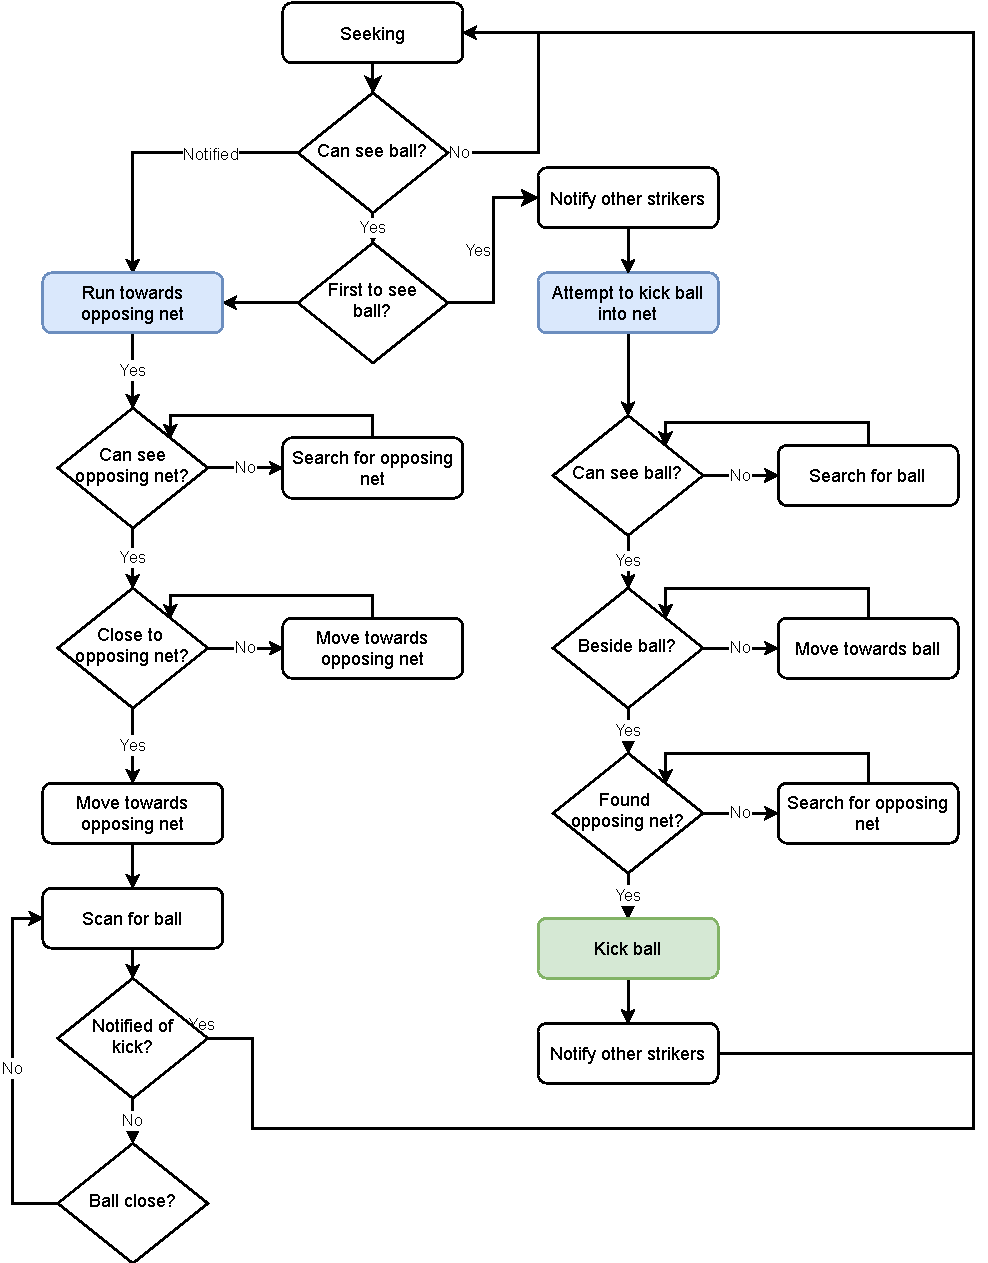
\includegraphics[scale=0.5]{fig/striker-flowchart.pdf}
		\caption{Flowchart for striker-type agents}
		\label{flowchart-striker}
	\end{figure}
	
	\begin{figure}[ht]
		\centering
		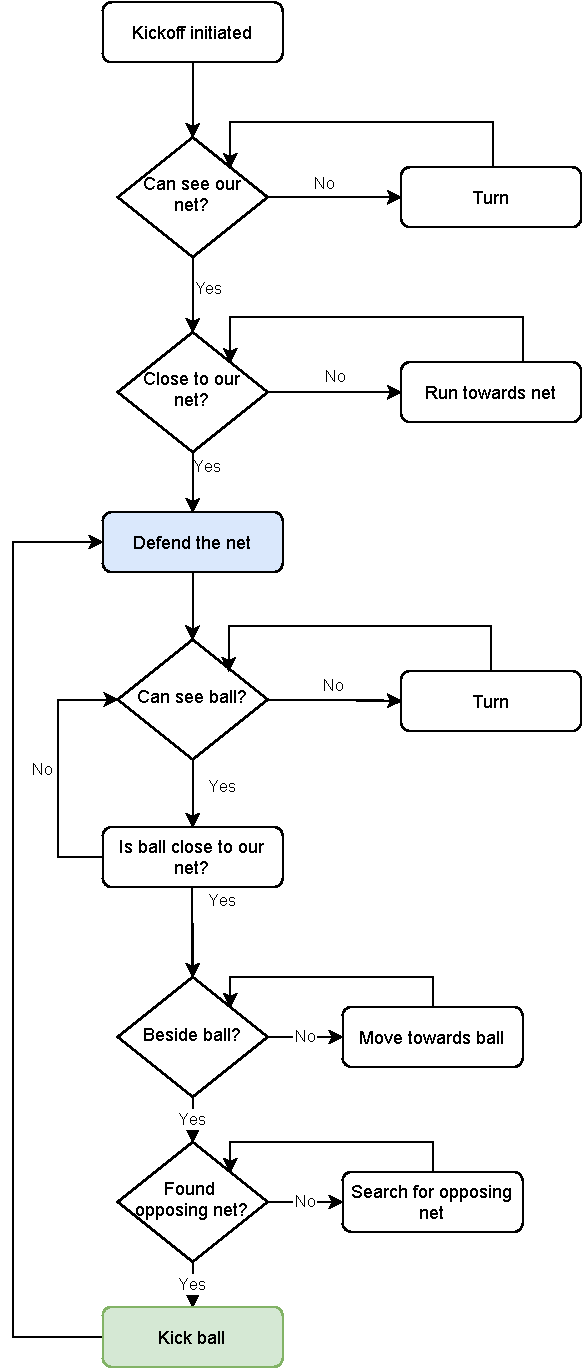
\includegraphics[scale=0.5]{fig/defender-flowchart.pdf}
		\caption{Flowchart for defender-type agents}
		\label{flowchart-defender}
	\end{figure}
	
	\subsection{Environment}
	The environment is a Java class that serves as the interface between the Robocup soccer environment server and the Jason framework. At program startup it initializes all Krislet objects and has callbacks to map Krislet memory objects to Jason percepts. 
	
	\subsection{Krislet}
	The Krislet program was provided as a demo agent to run in the Robocup simulation. This program was modified to be a stand alone agent for interfacing with the simulation, acting as a puppet for the Jason agent. Each Krislet object represents one Jason agent, and when created opens a socket to the soccer environment server and registers the player. Actions chosen by the Jason agent are executed by the Krislet object following the Command design pattern, which also feeds back percepts to the Jason agent.
	
	
	\section{Results}
	Basic functionality was first tested with the team playing standalone. One attacker successfully moved to the ball and others to the opposing net to support. Defenders moved to their own goal and waited for the ball to approach. After basic functionality was confirmed, a test game was played against a team of five default Krislet agents. Our team was reliably defeated by the default agents. While our solution was a good proof of concept, a few flaws became evident. Our Jason-controlled agents turn very slowly and have difficulty finding the ball. Attackers were able to keep the ball within their vision as they pursued it, but defenders struggled to find the ball before the default agent had already kicked it into the net. In addition, the most important task was to run after the ball and kick it into the target net but, due to the random nature of the movement speeds, with five default agents running after the ball, at least one of them usually arrived first, vastly outweighing the advantage of having agents open at the net. Finally, our agents only know how to kick the ball towards the opposing net, and do not account for opposing agents in the way; this leads to frequent interceptions by the opponents.
	
	\section{Conclusion}
	We implemented a team of agents that successfully coordinated to achieve their joint goal of scoring on the opposing side and preventing a goal on their net. Further development of this system would make the strikers properly communicate their distance to each other and have the closest agent move to the ball. Additionally the strikers should properly pass to other strikers rather than kick the ball directly at an opponent.
	
	
	\section{Appendix}
	\centering
	\begin{figure}[h]
		\centering
		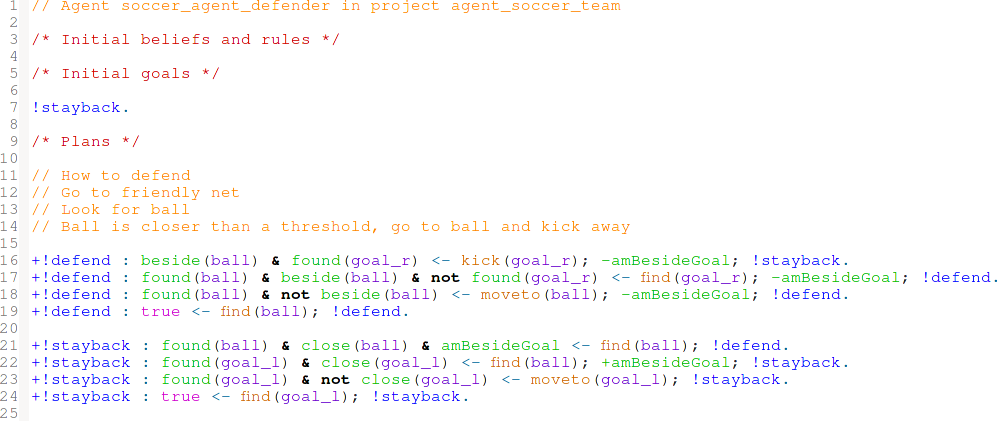
\includegraphics[width=0.8\textwidth]{fig/defender-code.png}
		\caption{AgentSpeak code for defender-type agents}
		\label{code-defender}
	\end{figure}
	
	\begin{figure}[h]
		\centering
		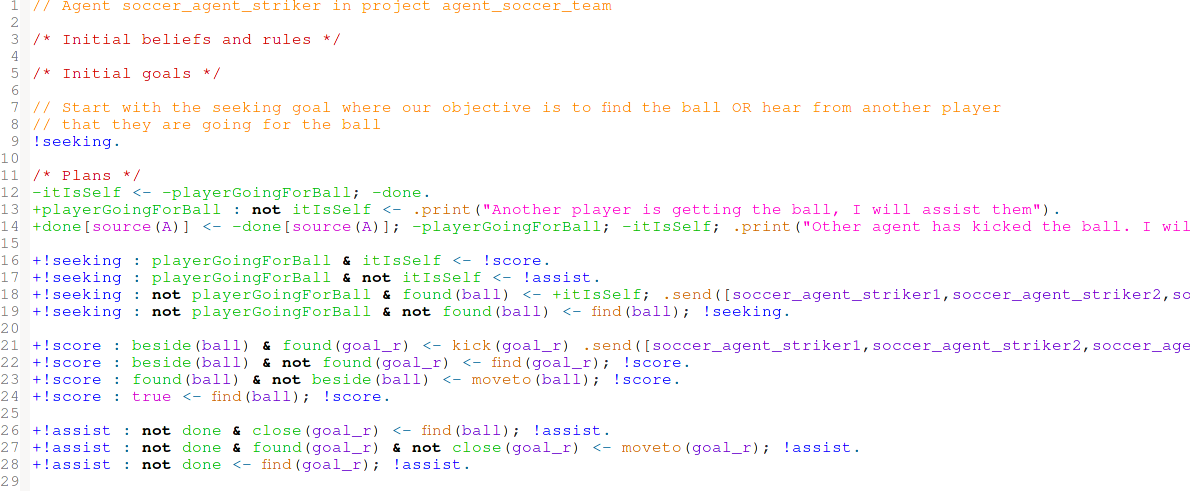
\includegraphics[width=0.8\textwidth]{fig/striker-code.png}
		\caption{AgentSpeak code for striker-type agents}
		\label{code-striker}
	\end{figure}
	
	
\end{document}
